tput/plots/Testing_data.pdf
Removing project1/output/plots/Testing_Ridge.pdf
Removing project1/output/plots/Testing_OLS_BV_compare_n170.pdf
Removing project1/output/plots/Testing_OLS_BV_compare_n169.pdf
Removing project1/output/plots/Testing_OLS.pdf
Removing project1/output/plots/SRTM_R2_OLS_n50_eps02_pol5.pdf
Removing project1/output/plots/SRTM_MSE_OLS_n50_pol5_Bootstrap_re50.pdf
Removing project1/output/plots/SRTM_MSE_OLS_n50_pol5_Bootstrap_re100.pdf
Removing project1/output/plots/SRTM_MSE_OLS_n50_pol50_Bootstrap_re50.pdf
Removing project1/output/plots/SRTM_MSE_OLS_n50_pol5.pdf
Removing project1/output/plots/SRTM_MSE_OLS_n50_pol10_CV_re5.pdf
Removing project1/output/plots/SRTM_MSE_OLS_n50_pol10_CV_re10.pdf
Removing project1/output/plots/SRTM_MSE_OLS_n500_pol5_Bootstrap_re100.pdf
Removing project1/output/plots/SRTM_MSE_OLS_n15_pol15_Bootstrap_re50.pdf
Removing project1/output/plots/SRTM_MSE_OLS_n15_pol1
	\endminipage\hfill
	\minipage{0.49\textwidth}
	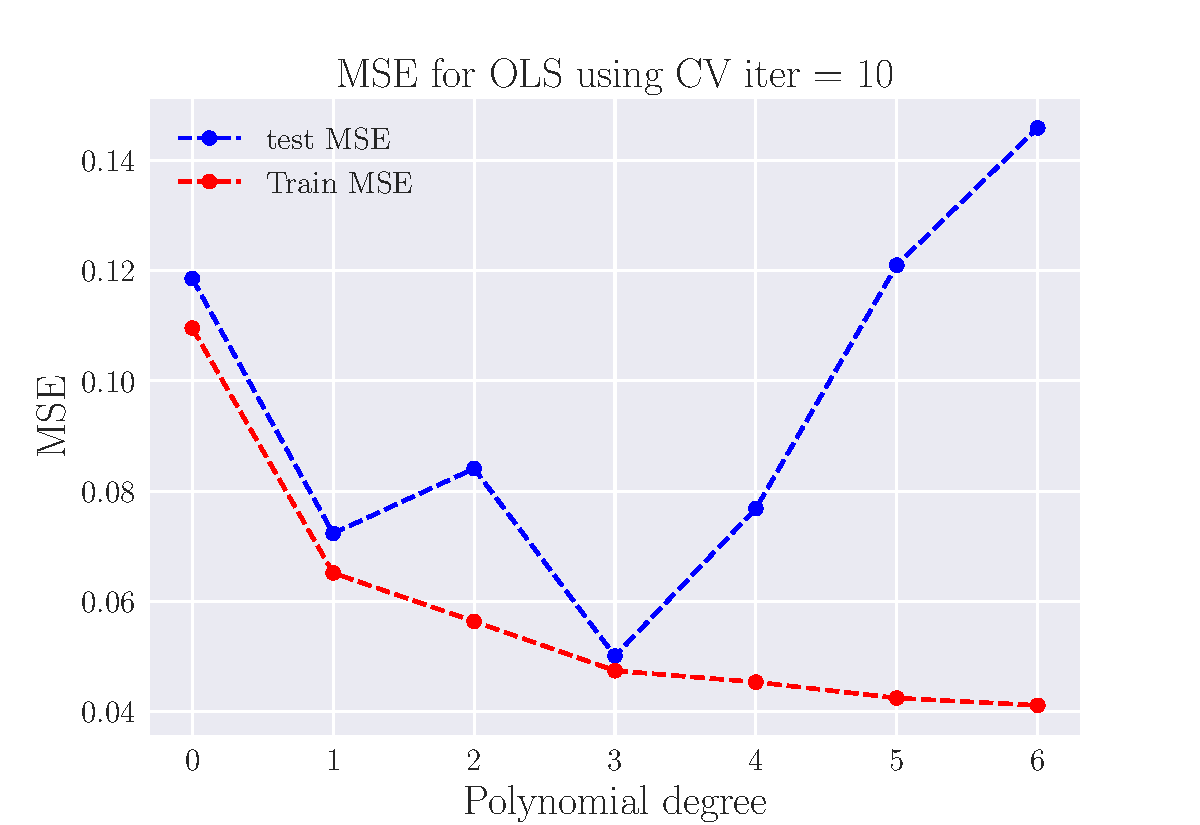
\includegraphics[width=\linewidth]{MSE_OLS_n30_eps02_pol6_CV_re10.pdf}
	\endminipage\hfill
	\minipage{0.49\textwidth}
	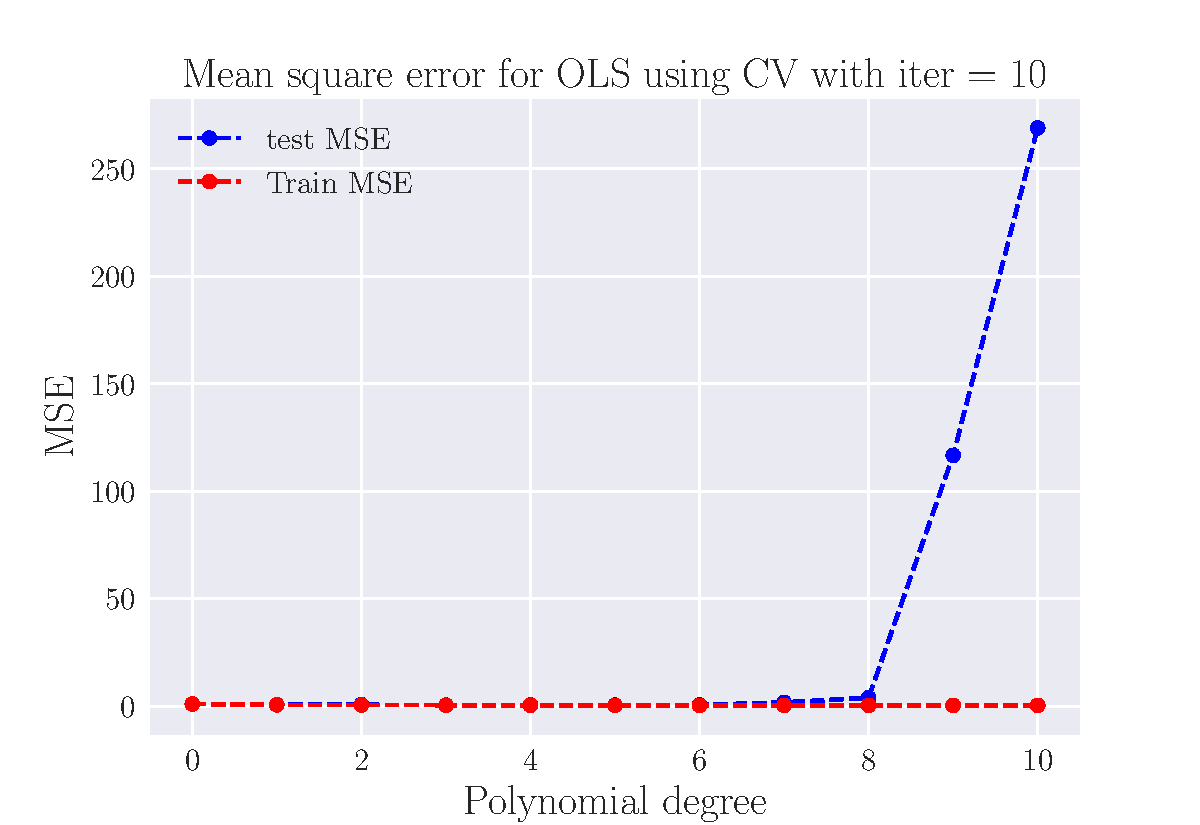
\includegraphics[width=\linewidth]{MSE_OLS_n30_eps02_pol10_CV_re10.pdf}
	\endminipage
	\caption{Here we have plotted the MSE when performing cross-validation as the resampling technique. On the $x$-axis we have polynomial degree, and MSE on the $y$-axis. The top left, right and bottom left figures are with $k=[5, 7, 10]$ iterations respectively. The bottom left plot is to illustrate the diverging MSE for higher polynomial degree, which we see irregardless of iteration-number.} \label{fig:CV_OLS}
\end{figure}

When bootstrapping we saw overfitting at around $p=6$. Looking at the plots in figure \ref{fig:CV_OLS} there seems to be consistent overfitting at around $p=3$. In the bottom right plot we have plotted for higher polynomials to illustrate that this error does not decrease for higher $p$. This does not depend on the number of resampling iterations. We see no obvious reason that the overfitting should start sooner compared to bootstrapping, and thus ground it in random fluctuations. We have consistently seen large variation in results based on number of resampling, and the random seed used when producing the results. Another interesting result is that a higher number of resampling iterations seems to decrease the overfitting effects. This coincide with the analysis on early overfitting. Having a larger number of resampling iterations should dampen the odd effects due to randomness.

\section*{Exercise 4: Ridge Regression on the Franke function with resampling}
In some cases, it might happen that the matrix $\mathbf{X}^T\mathbf{X}$ is singular, such that it is non-invertible. This is the case if some of the independent variables are highly correlated. Then OLS will not work, see \eqref{eq:OLS_beta}. However, by adding a small number $\lambda$ to the diagonal, the matrix is no longer singular. This is called Ridge regression. The optimal parameters $\boldsymbol{\hat\beta}$ are given by
\begin{equation}
	\boldsymbol{\hat{\beta}} = (X^TX+\lambda I)X^T\vc{z},
\end{equation}
where $I$ is  the identity matrix. The parameter $\lambda$ can take any value, so finding the optimal is paramount. This is done by running the regression for many different values of $\lambda$ and choosing the one giving the best results.  Note that when $\lambda=0$, the expression becomes that of OLS.

Now we want to perform the same bootstrap analysis as we did for OLS, using Ridge. Here we also take a look at when we have overfitting, for different values of $\lambda$ and with bootstrap. Figure \ref{fig:Ridge_boot_PM} shows MSE as function of polynomial degree for 4 different values of $\lambda$, starting at $10^-4$, increasing with a factor of 100 for each plot. We see that test error varies a lot, making it non-trivial to determine what is overfitting and underfitting. For the 3 first $\lambda$-values it seems we have overfitting for $p=9$, while for $\lambda=100$, it can not be conclusively decided. $p=3$ and $p=8$ seem to be the best two values before overfitting for the 3 smallest $\lambda$.

\begin{figure}[H]
	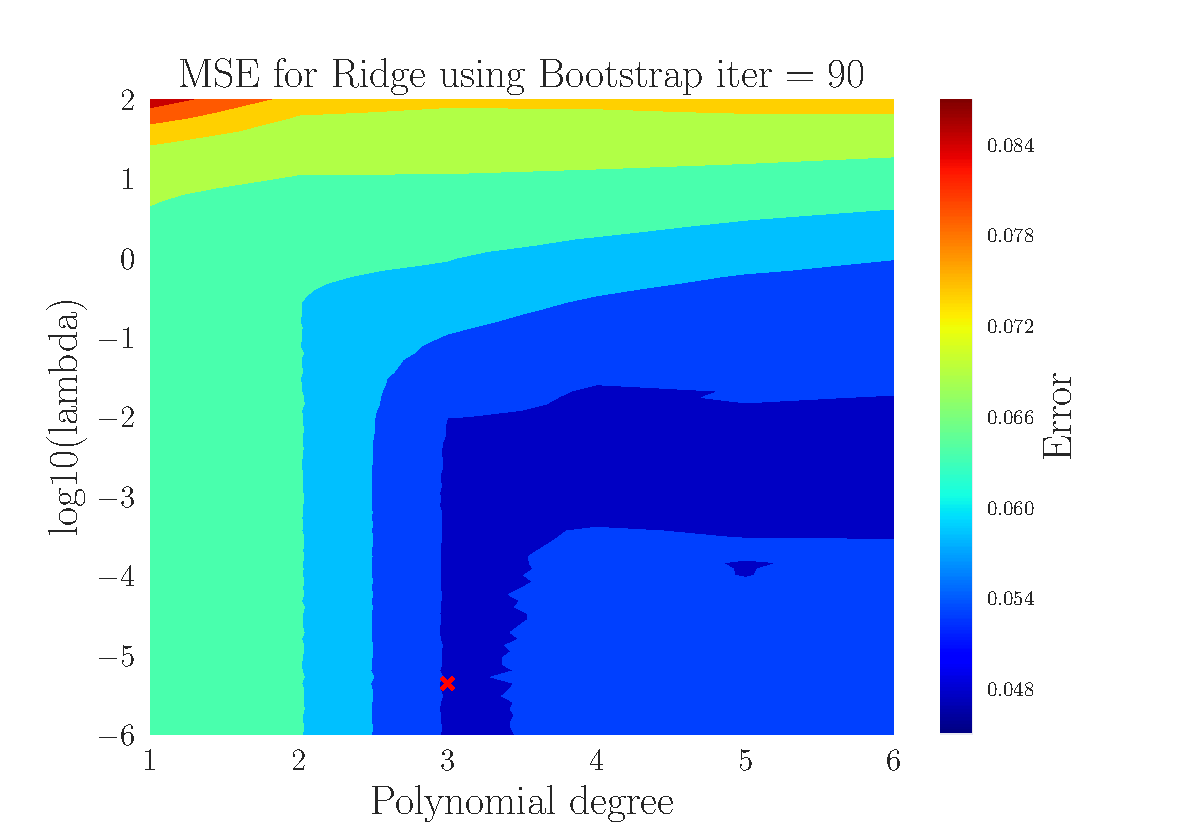
\includegraphics[width=\linewidth]{Contour_PL_Ridge_Bootstrap90_n30_eps0.2_p1_6_lmb2_m6.pdf}
	\caption{MSE using Ridge and bootstrapping, as function of polynomial degree and $\lambda$. The minimum value is $MSE=0.047$ at $p=3$ and $log10(\lambda) = -4.4$.}
	\label{fig:Ridge-boot_heatmap}
\end{figure}

\begin{figure}[H]
	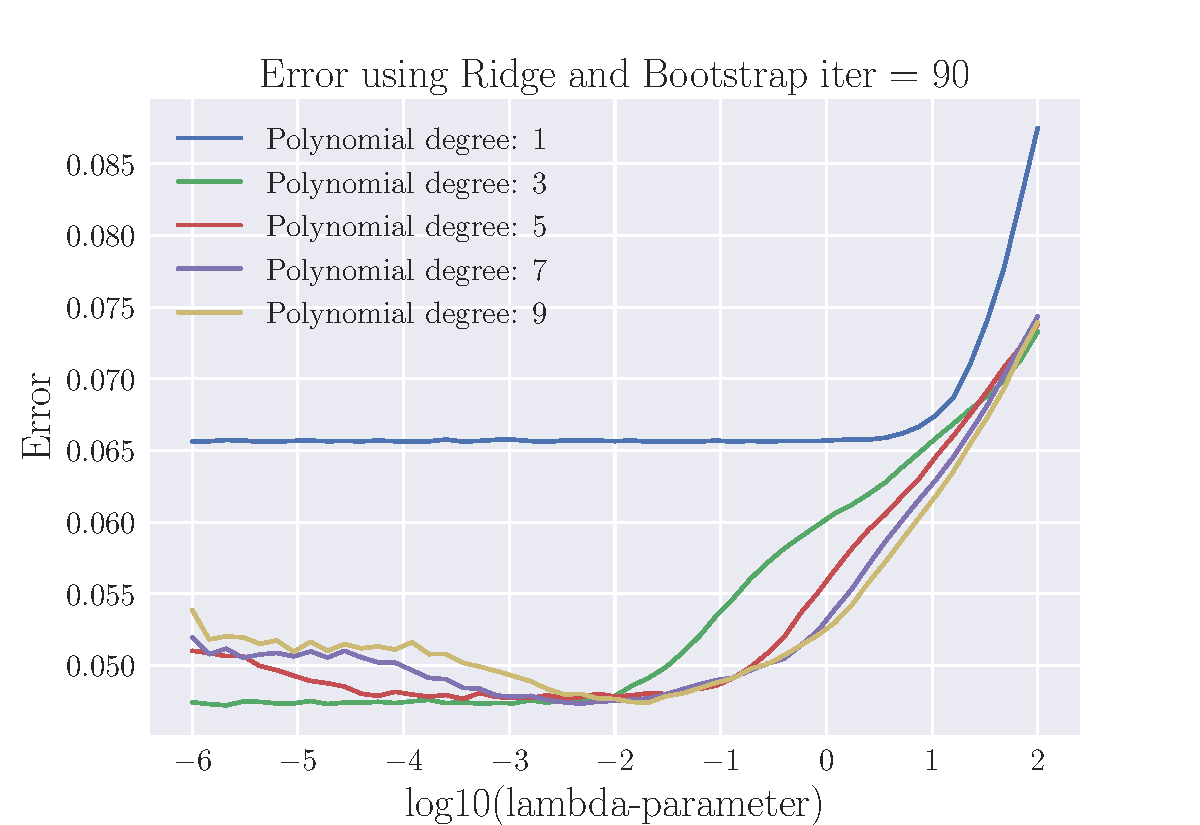
\includegraphics[width=\linewidth]{lambdaMSE_Ridge_Bootstrap90_n30_eps02_p9_lm6_2.pdf}
	\caption{MSE using Ridge and bootstrapping, as function of $\lambda$ for different polynomial degrees.}
	\label{fig:Ridge-boot_heatmap}
\end{figure}


\begin{figure}[H]
	\minipage{0.49\textwidth}
	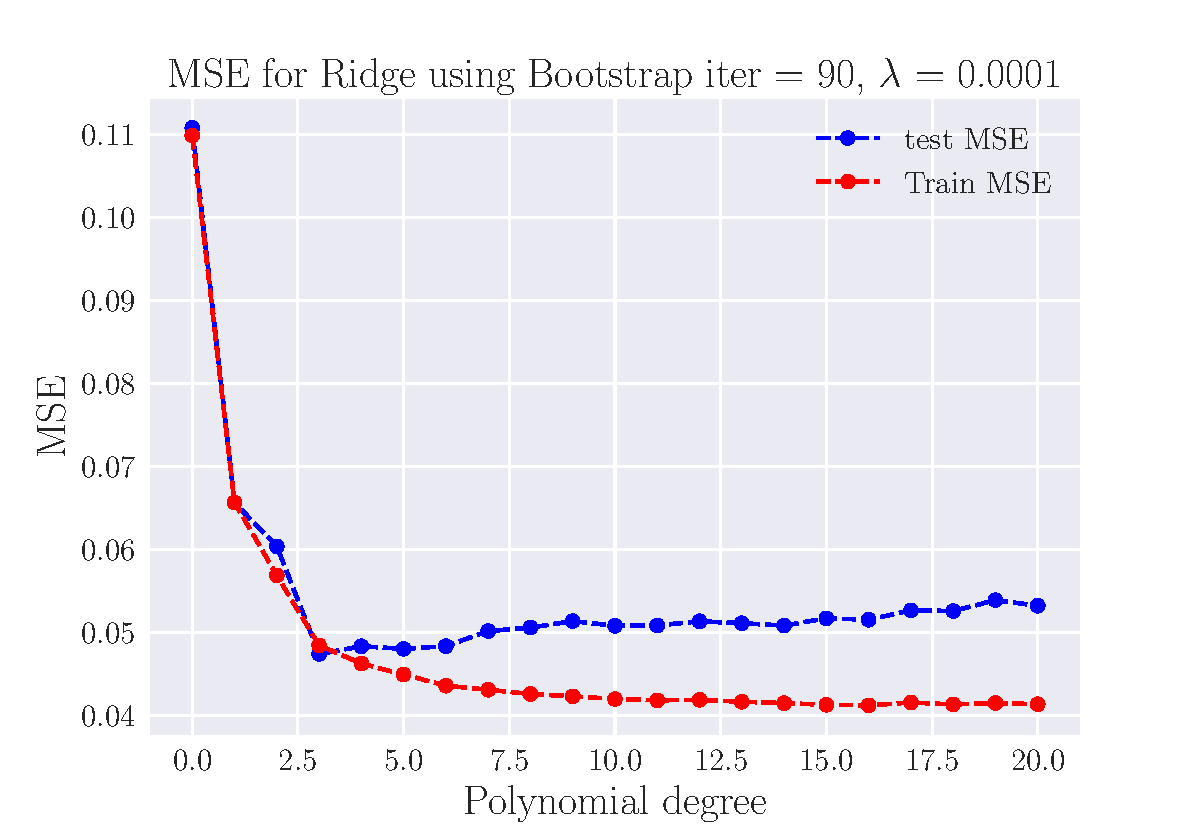
\includegraphics[width=\linewidth]{MSE_Ridge_n30_eps02_pol20_Bootstrap_re90_lam_0_0001.pdf}
	\endminipage\hfill
	\minipage{0.49\textwidth}
	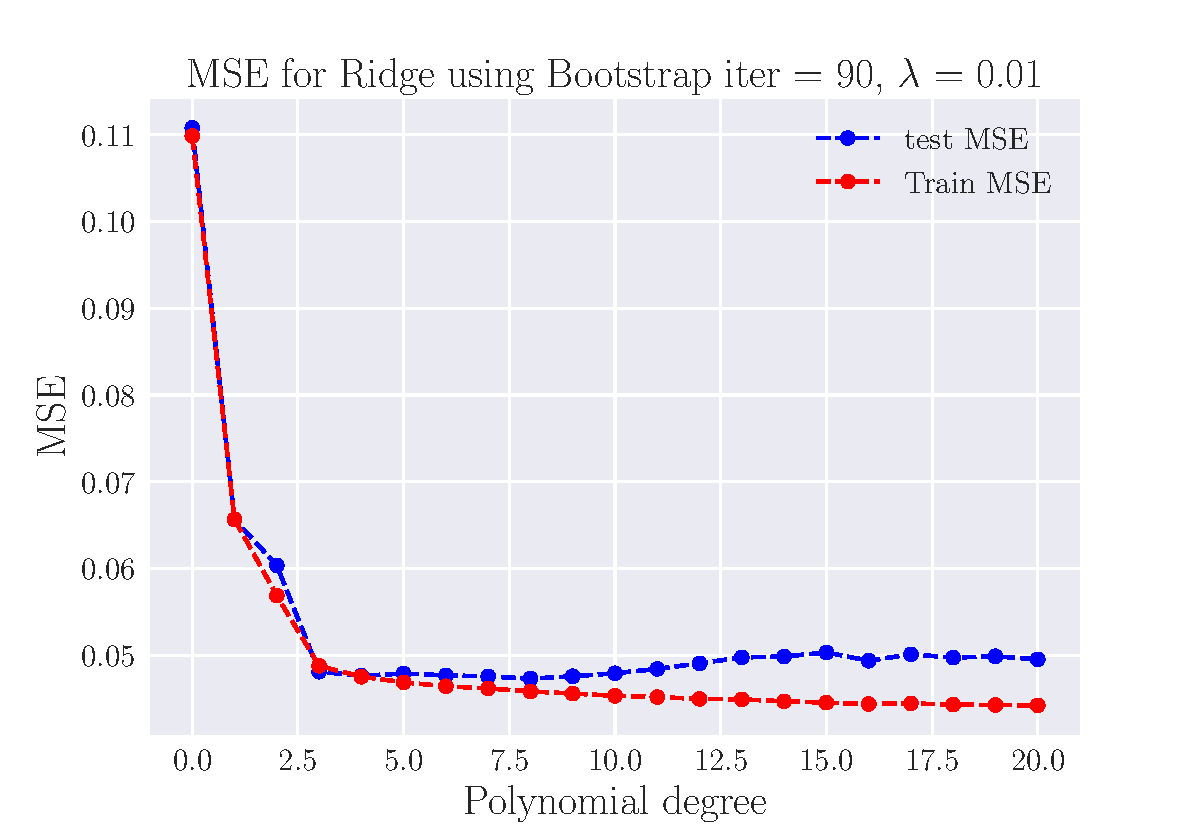
\includegraphics[width=\linewidth]{MSE_Ridge_n30_eps02_pol20_Bootstrap_re90_lam_0_01.pdf}
	\endminipage\hfill
	\minipage{0.49\textwidth}
	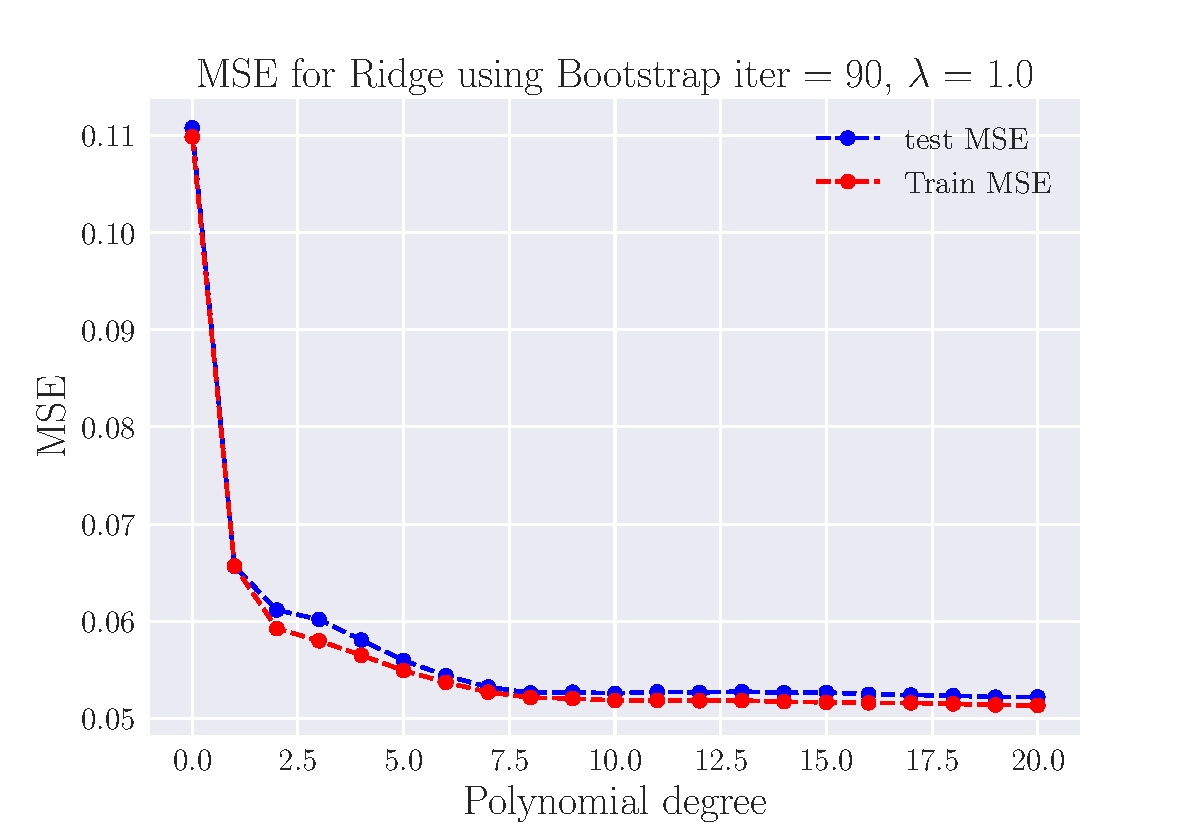
\includegraphics[width=\linewidth]{MSE_Ridge_n30_eps02_pol20_Bootstrap_re90_lam_1_0.pdf}
	\endminipage\hfill
	\minipage{0.49\textwidth}
	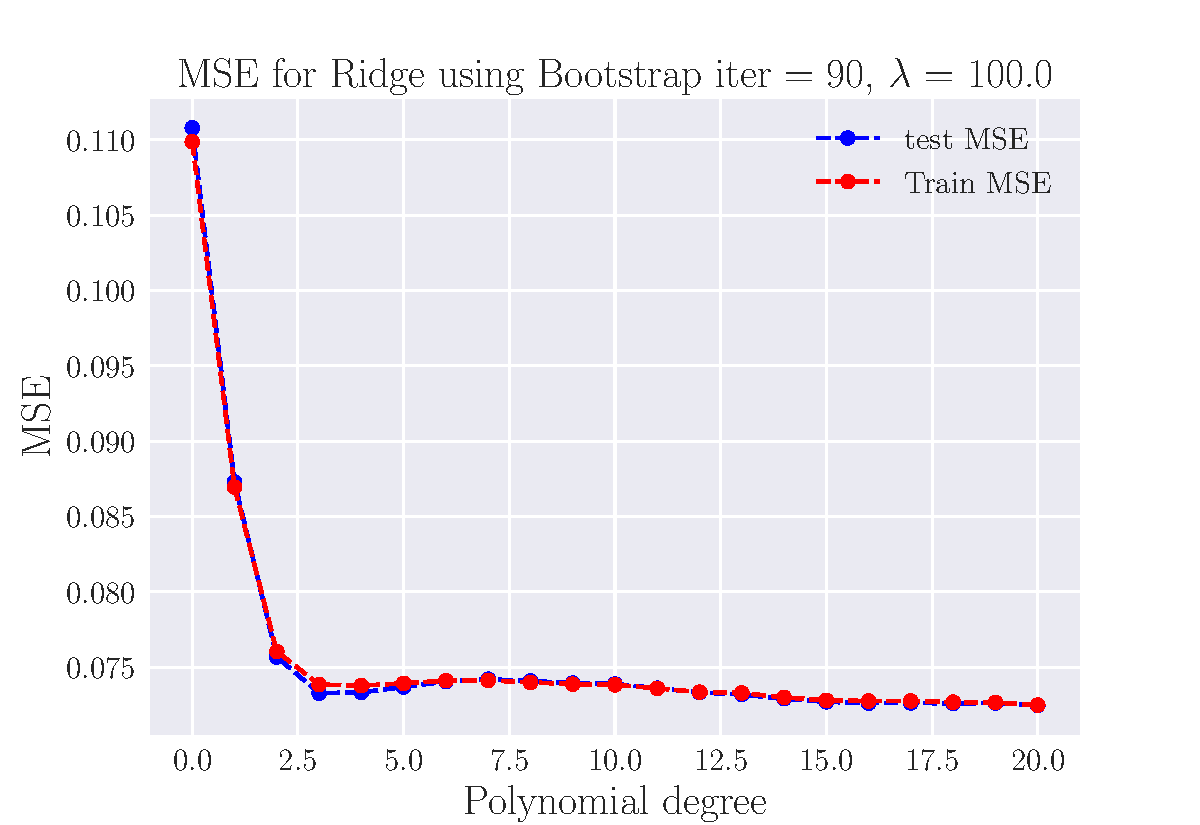
\includegraphics[width=\linewidth]{MSE_Ridge_n30_eps02_pol20_Bootstrap_re90_lam_100_0.pdf}
	\endminipage
	\caption{MSE using Ridgeregression and bootstrapping, as function of complexity, for different values of $\lambda$.} \label{fig:Ridge_boot_PM}
\end{figure}

To explore the $\lambda$-dependence more in-depth, we now choose a single polynomial degree and  plot the error as function of $\lambda$.  In figure \ref{fig:Ridge_boot_LM} we have done this for the two values noted above,$p=3$ and $p=8$.
q

\begin{figure}[H]
	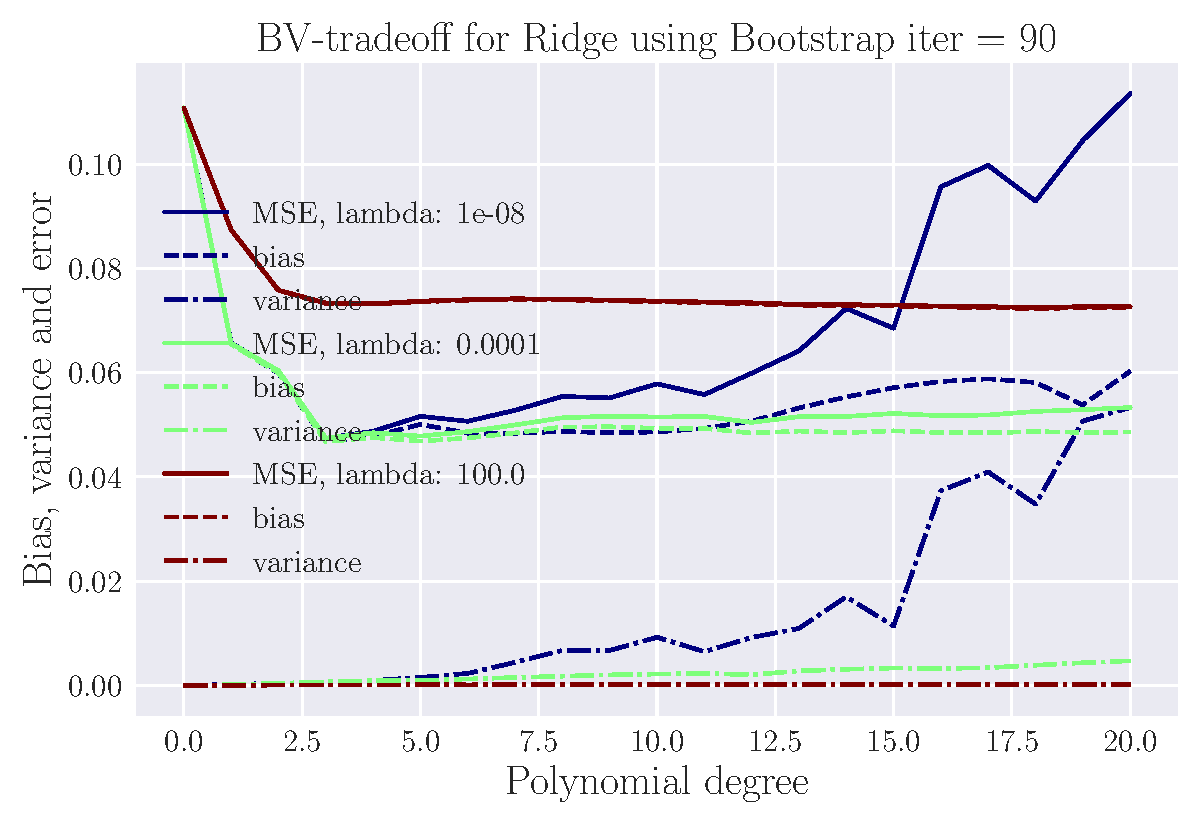
\includegraphics[width=\linewidth]{LBVT_Ridge_Bootstrap_n30_eps0_2_p20_lmbm8_2.pdf}
	\caption{MSE using Ridge and bootstrapping, as function of $\lambda$ for different polynomial degrees.}
	\label{fig:Ridge_boot_BVT}
\end{figure}

\begin{figure}[H]
	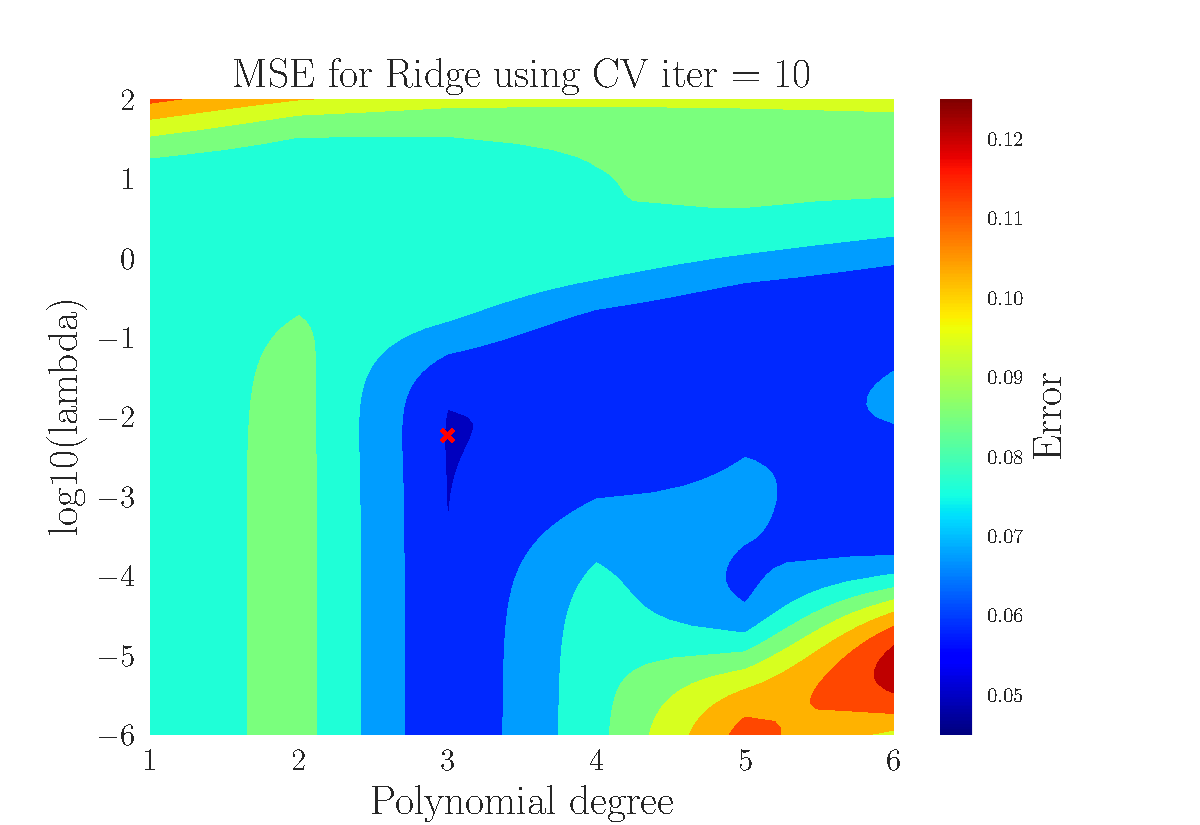
\includegraphics[width=\linewidth]{Contour_PL_Ridge_CV10_n30_eps0.2_p1_6_lmb2_m6.pdf}
	\caption{MSE using Ridge and bootstrapping, as function of $\lambda$ for different polynomial degrees.}
	\label{fig:Ridge_boot_BVT}
\end{figure}

\begin{figure}[H]
	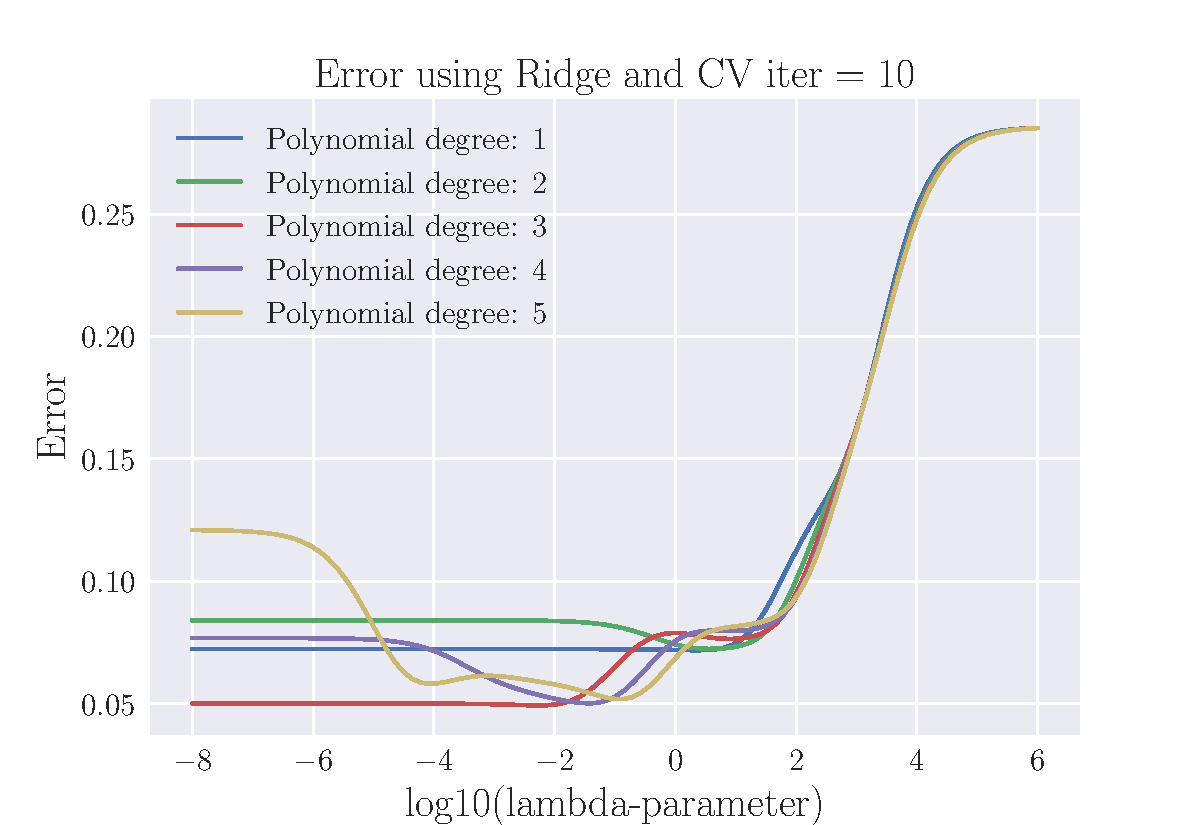
\includegraphics[width=\linewidth]{lambdaMSE_Ridge_CV10_n30_eps02_p5_lm8_6.pdf}
	\caption{MSE using Ridge and bootstrapping, as function of $\lambda$ for different polynomial degrees.}
	\label{fig:Ridge_boot_BVT}
\end{figure}


\begin{figure}[H]
	\minipage{0.49\textwidth}
	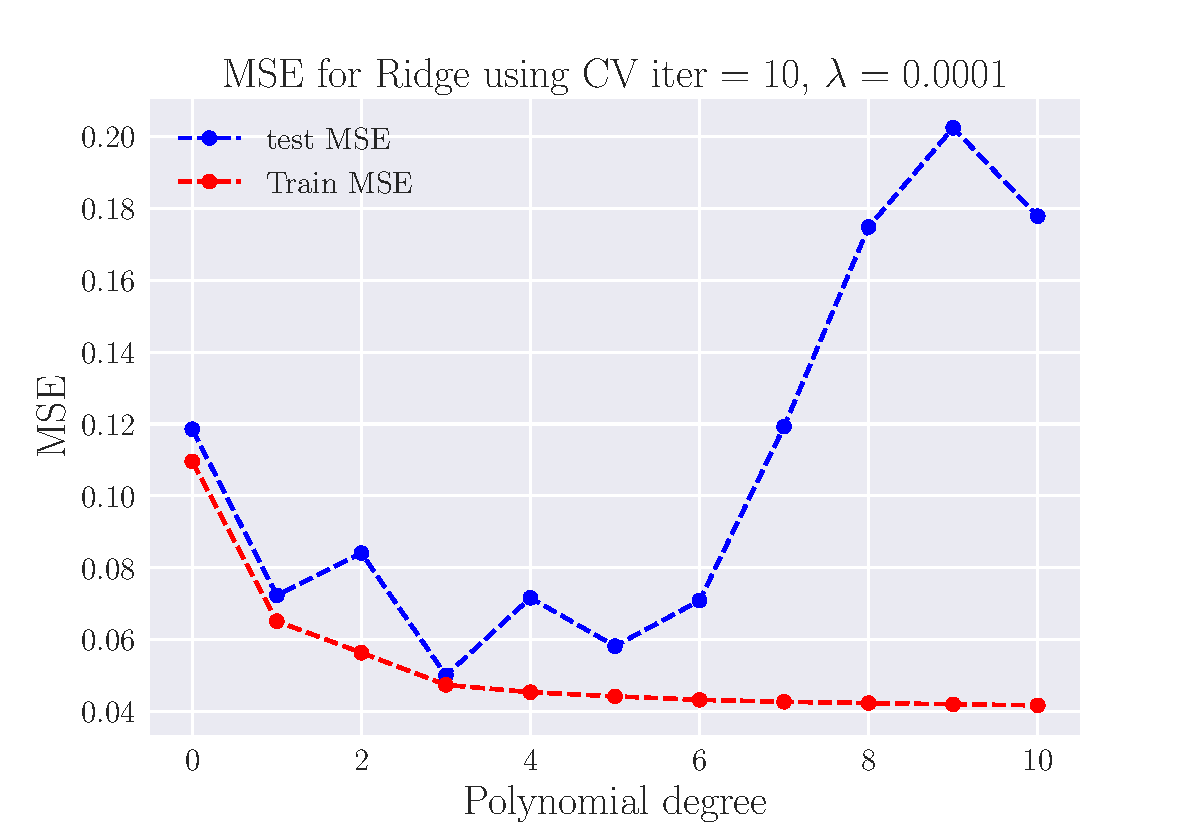
\includegraphics[width=\linewidth]{MSE_Ridge_n30_eps02_pol10_CV_re10_lam_0_0001.pdf}
	\endminipage\hfill
	\minipage{0.49\textwidth}
	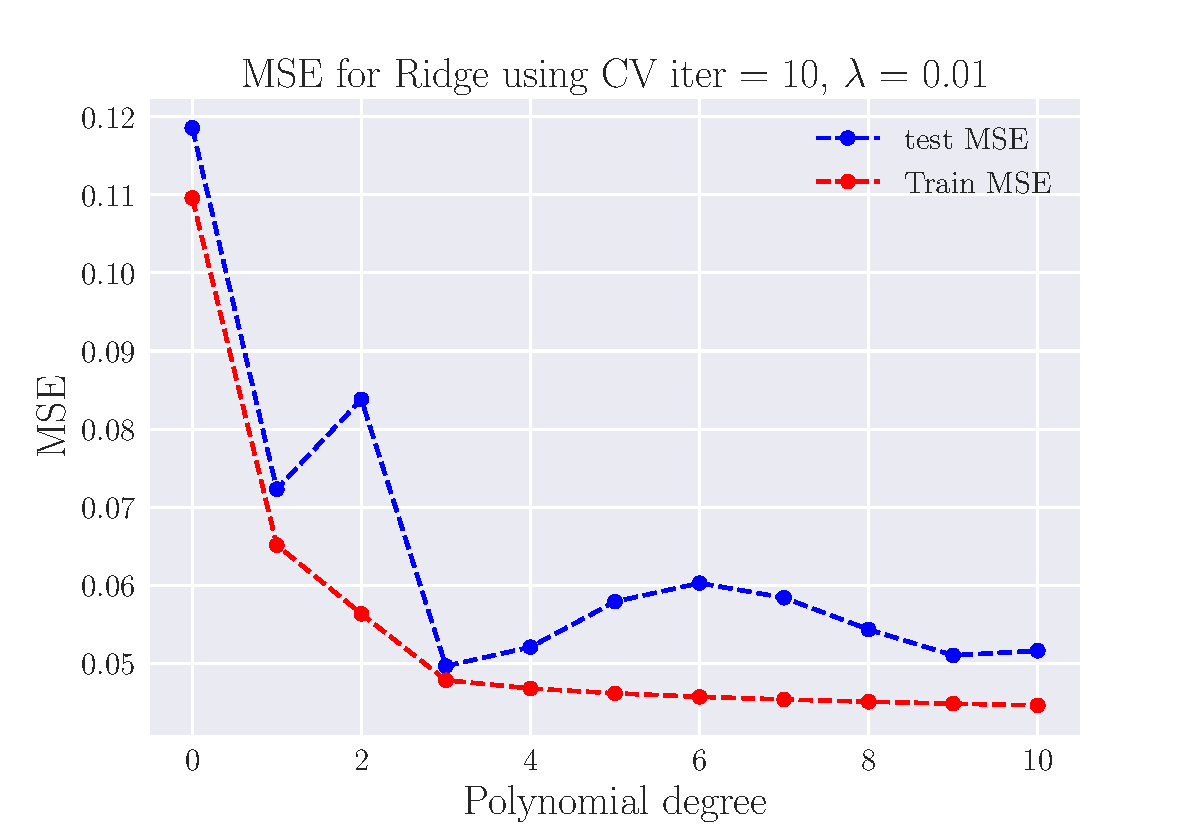
\includegraphics[width=\linewidth]{MSE_Ridge_n30_eps02_pol10_CV_re10_lam_0_01.pdf}
	\endminipage\hfill
	\minipage{0.49\textwidth}
	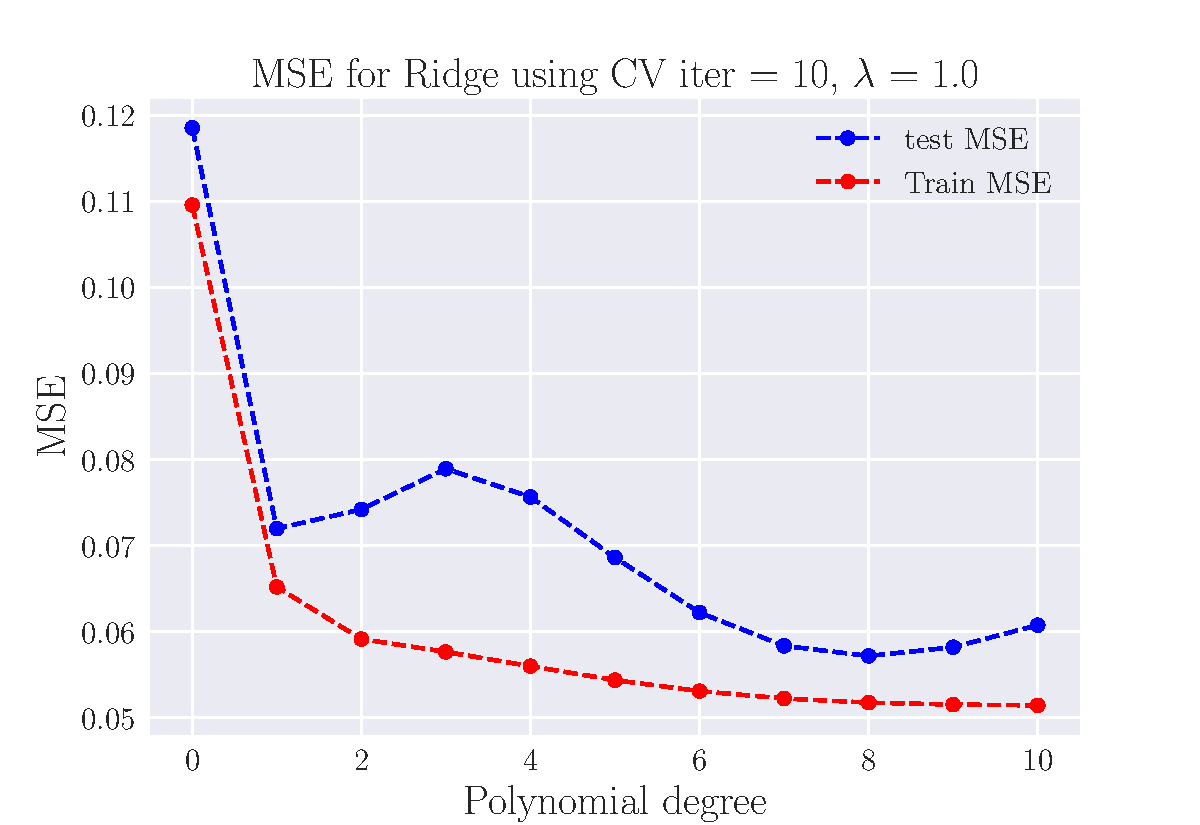
\includegraphics[width=\linewidth]{MSE_Ridge_n30_eps02_pol10_CV_re10_lam_1_0.pdf}
	\endminipage\hfill
	\minipage{0.49\textwidth}
	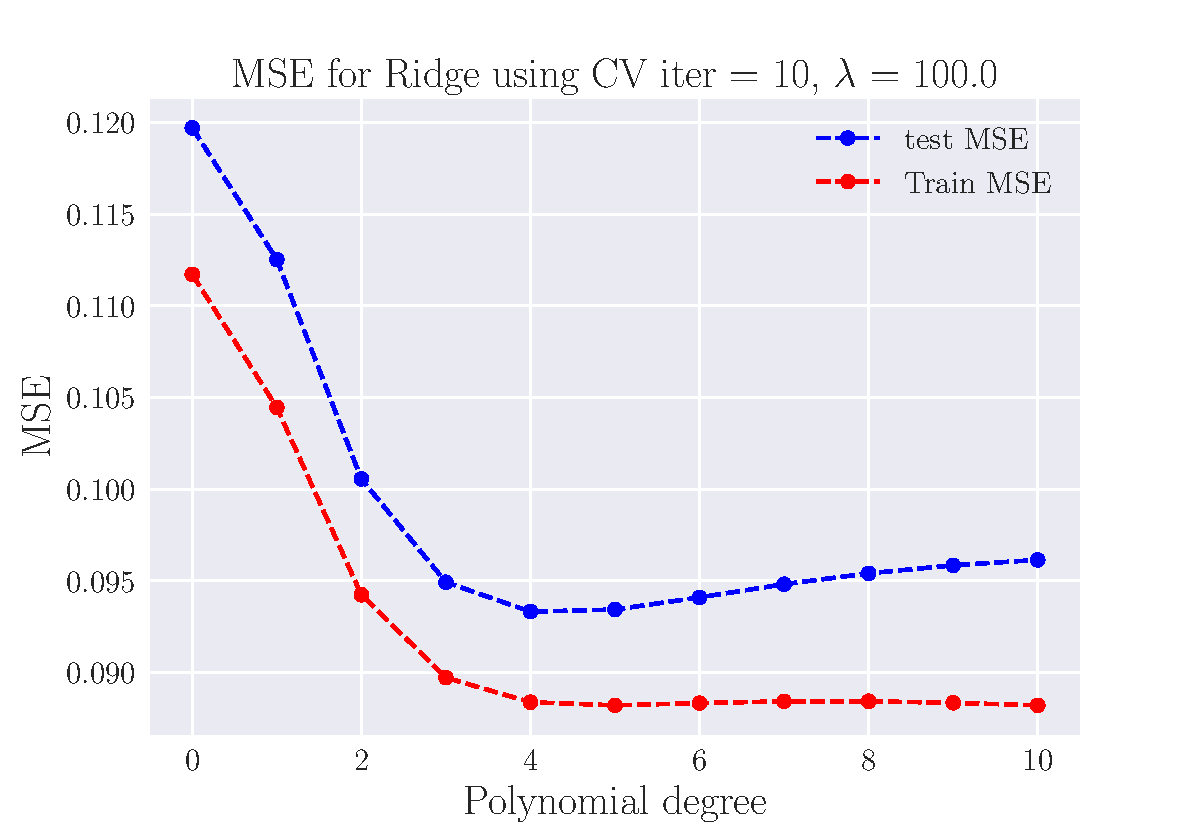
\includegraphics[width=\linewidth]{MSE_Ridge_n30_eps02_pol10_CV_re10_lam_100_0.pdf}
	\endminipage
	\caption{MSE using Ridgeregression and cross-validation, as function of complexity, for different values of $\lambda$.} \label{fig:Ridge_CV_PM}
\end{figure}


\section*{Exercise 5: Lasso regression on the Franke function with resampling}

\begin{figure}[H]
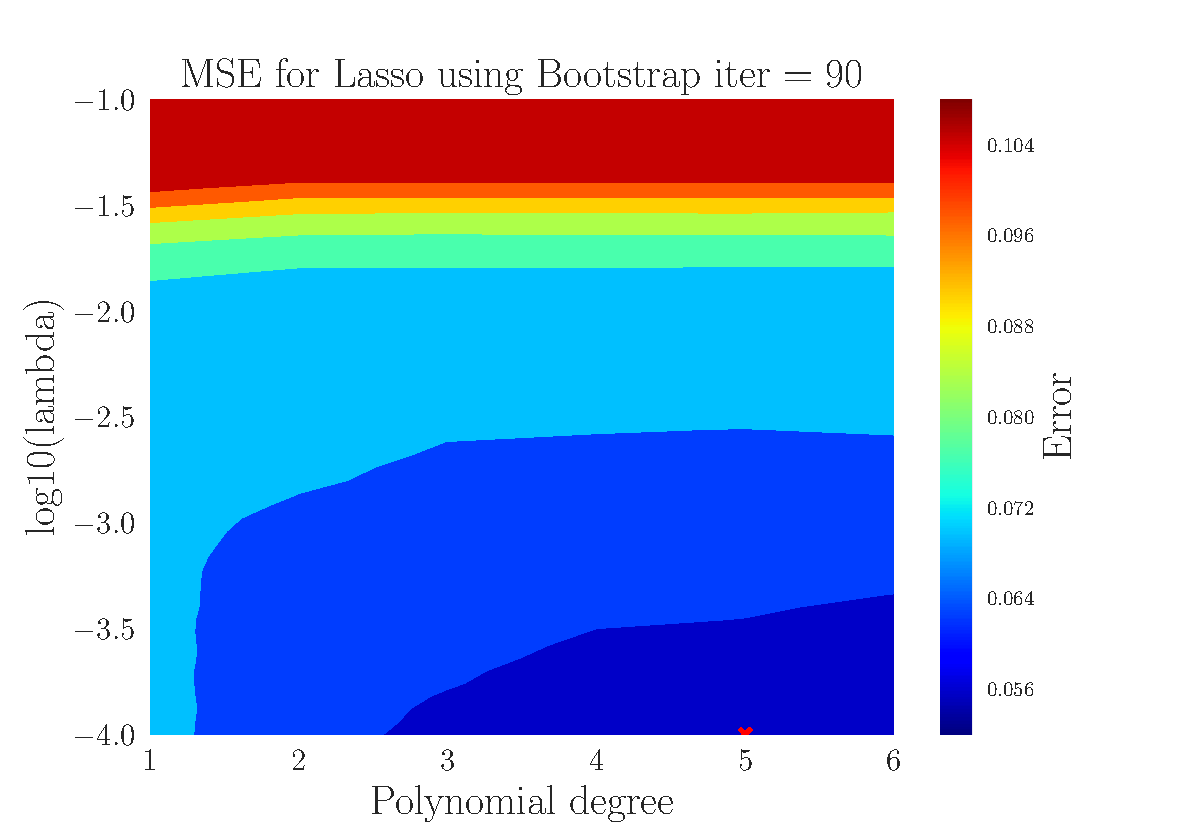
\includegraphics[width=\linewidth]{Contour_PL_Lasso_Bootstrap90_n30_eps0.2_p1_6_lmbm1_m4.pdf}
\caption{MSE using Ridge and bootstrapping, as function of $\lambda$ for different polynomial degrees.}
\label{fig:Ridge_boot_BVT}
\end{figure}


\begin{figure}[H]
	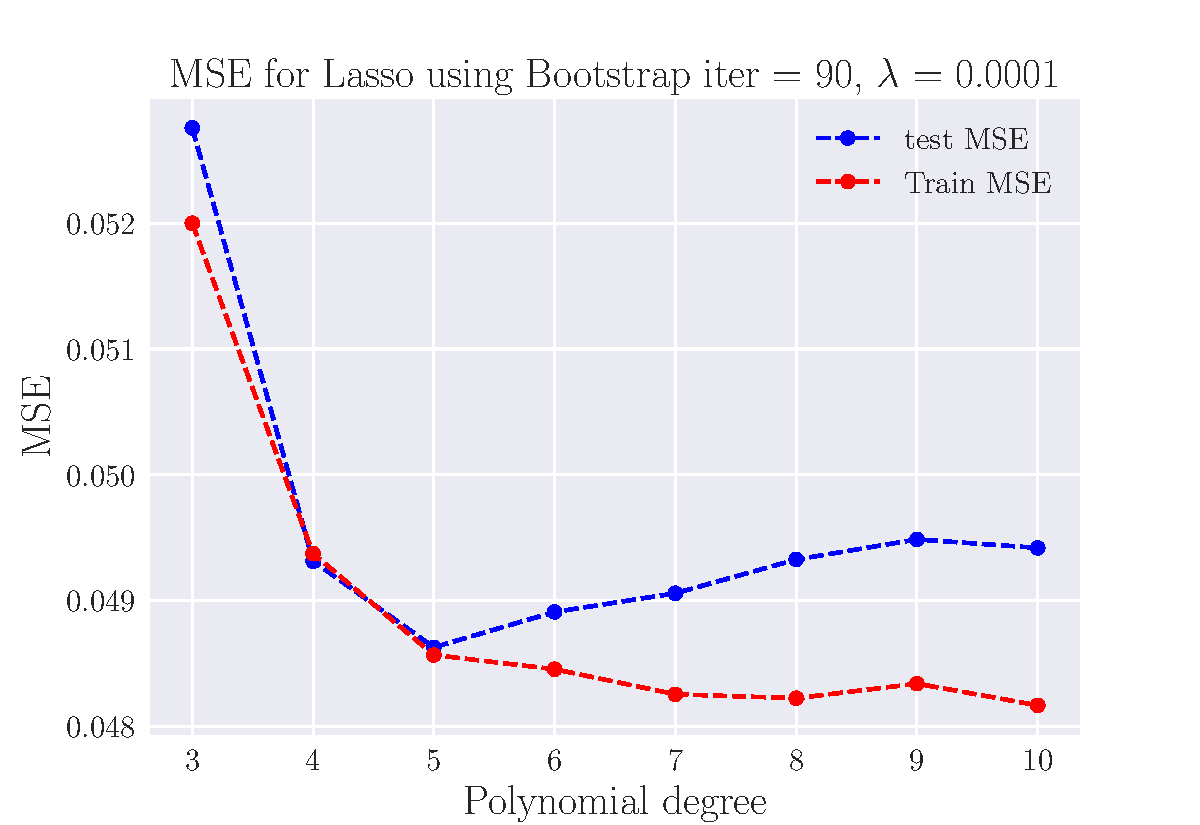
\includegraphics[width=\linewidth]{MSE_Lasso_n30_eps02_pol10_Bootstrap_re90_lam_0_0001.pdf}
	\caption{MSE using Ridge and bootstrapping, as function of $\lambda$ for different polynomial degrees.}
	\label{fig:Ridge_boot_BVT}
\end{figure}



\section*{Exercise 6: Analysis of real data}

Having used our data analysis methods to study the Franke function we will now move on to study data from the real world. We will consider Norwegian terrain data from here\footnote{\href{https://github.com/CompPhysics/MachineLearning/tree/master/doc/Projects/2021/Project1/DataFiles}{https://github.com/CompPhysics/MachineLearning/tree/master/doc/Projects/2021/Project1/DataFiles}}. Because the datasets are large, we will only consider one small part of \texttt{SRTM\_data\_Norway\_1.tif}, namely $f_{i,j}$ where $i,j\in[50,100]$, i.e. $N=50$ datapoints in each direction. It is useful to consider dimensionless data, thus we divide by the highest point $z_{i,j} = f_{i,j}/\max{|f_{i,j}|}$, and let $i,j\in[50,100] \rightarrow x,y\in[0,1]$ when plotting. Then we get the data visualized in figure \ref{fig:terrain_raw}.

\begin{figure}[H]
  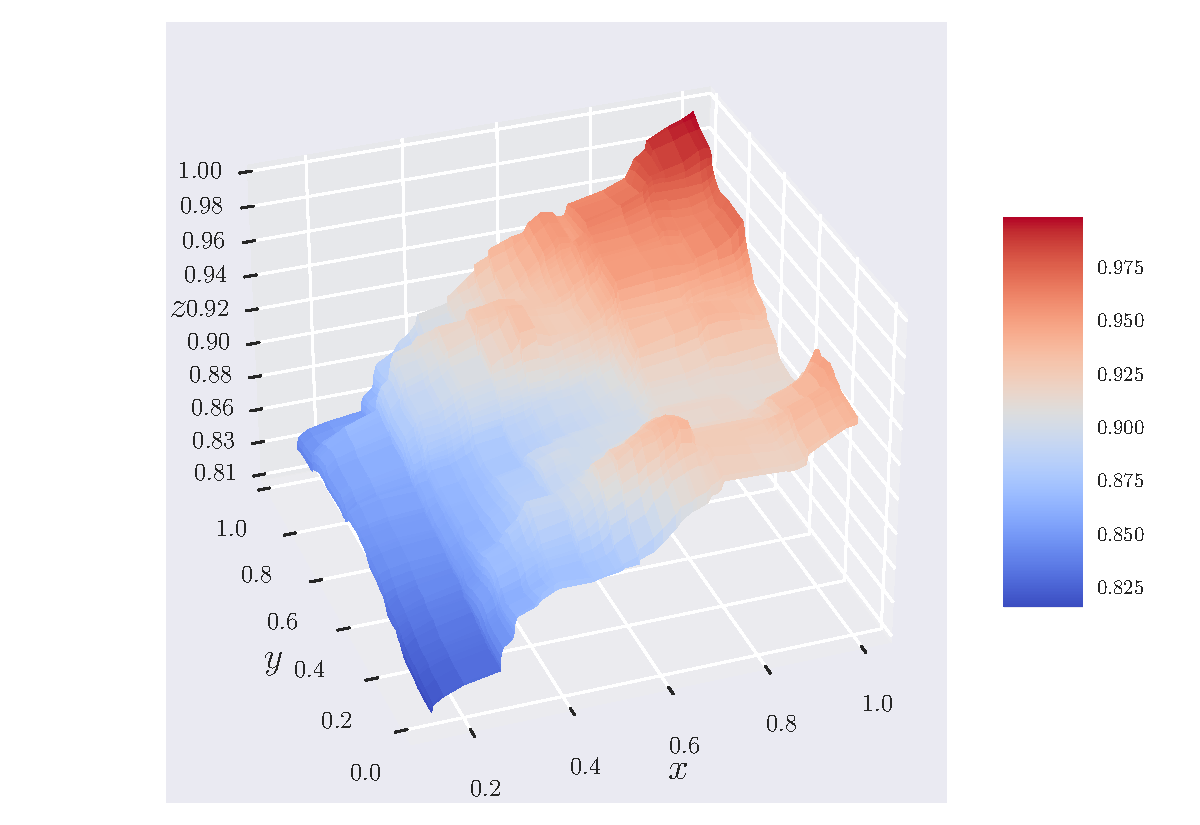
\includegraphics[width=\linewidth]{SRTM_rawdata_n50.pdf}
  \caption{Here we have plotted the terrain data which we will use in this exercise.}
  \label{fig:terrain_raw}
\end{figure}

We begin by studying the MSE using OLS-regression and bootstrapping as the resampling technique. Our results should mirror those we got in exercise 2, where the test MSE decreases in the beginning, and increases when we start overfitting. Choosing $B = 50$ iterations and max polynomial degree $p_\text{max} = 30$ we get the MSE illustrated in figure \ref{fig:terrain_OLS_MSE_bootstrap}. Because of the small variation in MSE we plotted the $\log(\text{MSE})$ along the $y$-axis.

\begin{figure}[H]
  \minipage{0.49\textwidth}
  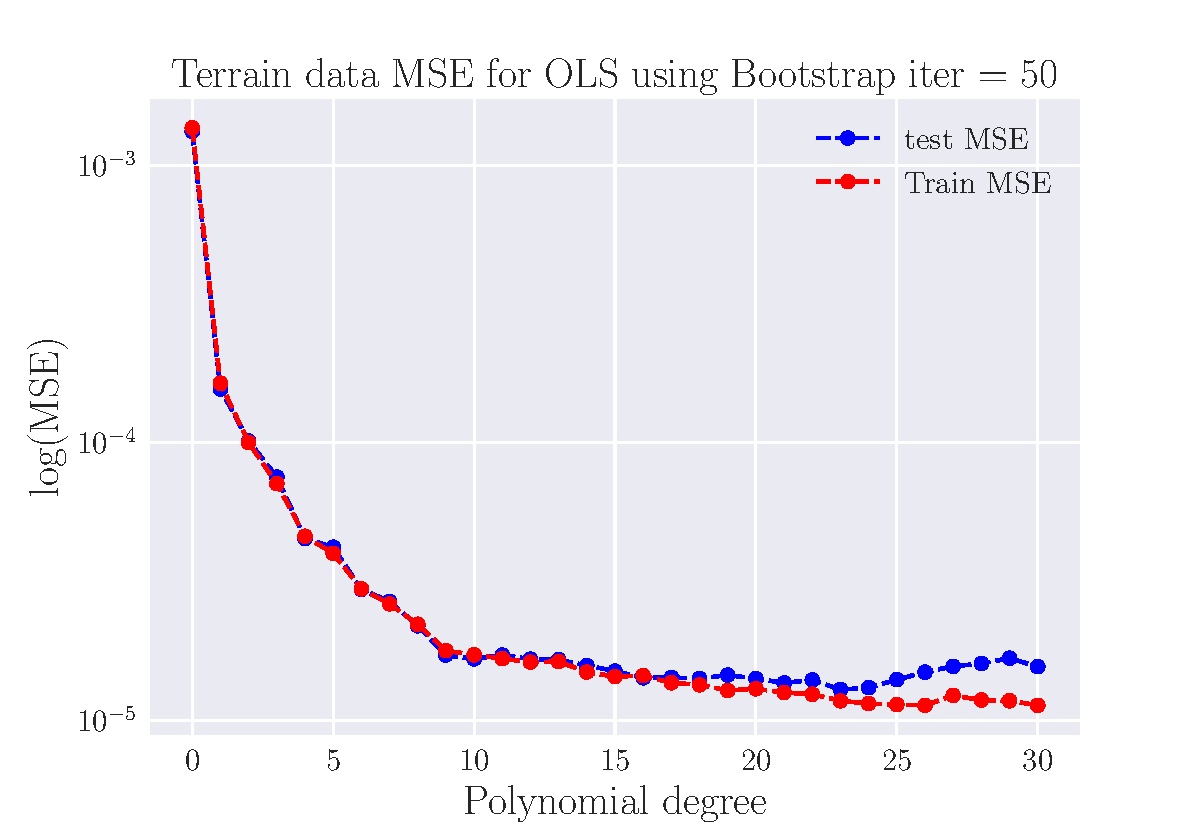
\includegraphics[width=\linewidth]{SRTM_MSE_OLS_n50_pol30_Bootstrap_re50_log.pdf}
  \endminipage\hfill
  \minipage{0.49\textwidth}
  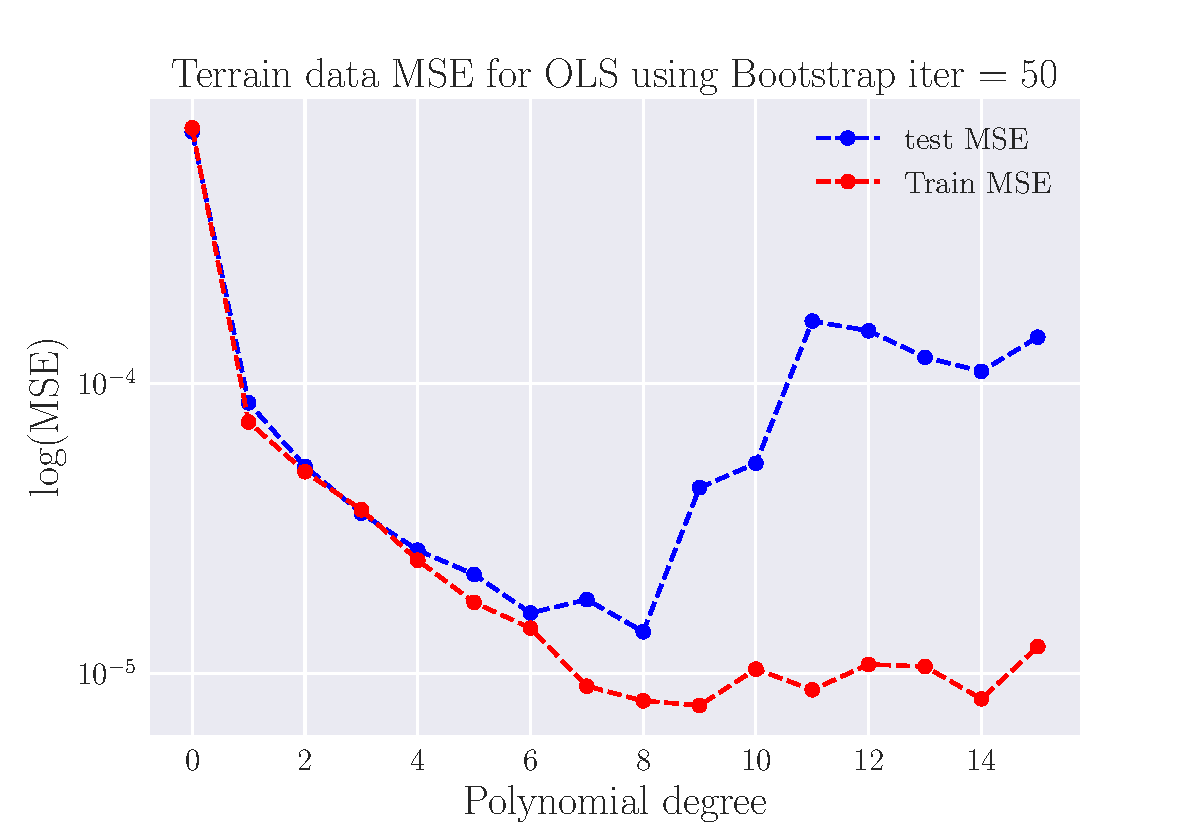
\includegraphics[width=\linewidth]{SRTM_MSE_OLS_n30_pol15_Bootstrap_re50_log.pdf}
  \endminipage
  \caption{Her we have plotted the $\log(\text{MSE})$ as a function of polynomial degree. The left plot is with $(50\cross50)$ grid-points and right with $(30\cross30)$.}
  \label{fig:terrain_OLS_MSE_bootstrap}
\end{figure}

Looking at figure \ref{fig:terrain_OLS_MSE_bootstrap} we see that for $(50\cross50)$ grid-points (left plot), we get a small increase in the MSE after $p = 23$. We think this is because of the large number of grid points. Therefore we plot for $30\cross30$ grid-points (right figure) and see a much larger increase after $p = 8$. Because of this we conclude that the small overfitting is due to our large number of grid-points.

As a simple sanity check, we plot the result of our fits for different polynomial degrees, which we can compare to the original data from figure \ref{fig:terrain_raw}. To capture the complexity of our data set, we consider four polynomial degrees, using $p\in[10,\,20,\,30,\,50]$, where the first two are shown in the upper left and right panel of figure \ref{fig:terrain_fit}, respectively, while the latter two in the bottom left and right panel of the same figure, respectively.

\begin{figure}[H]
	\minipage{0.49\textwidth}
	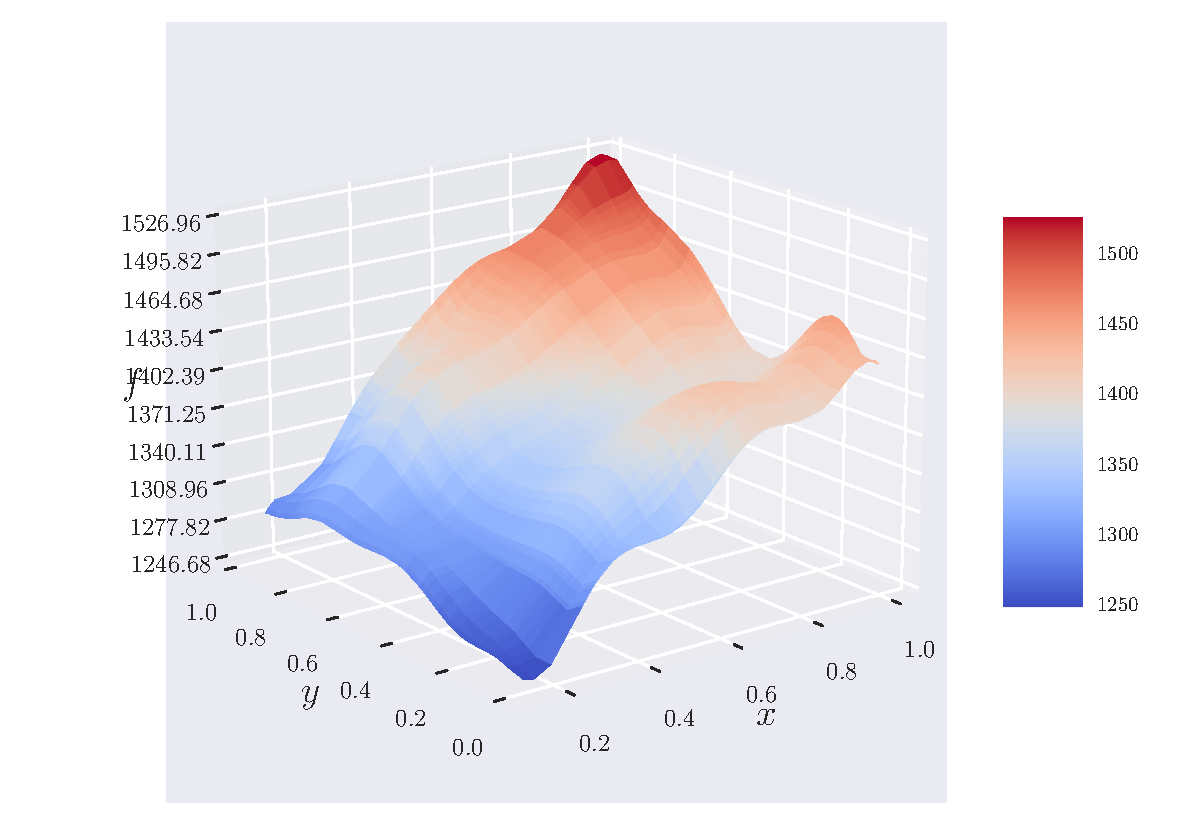
\includegraphics[width=\linewidth]{SRTM_prediction_p10.pdf}
	\endminipage\hfill
	\minipage{0.49\textwidth}
	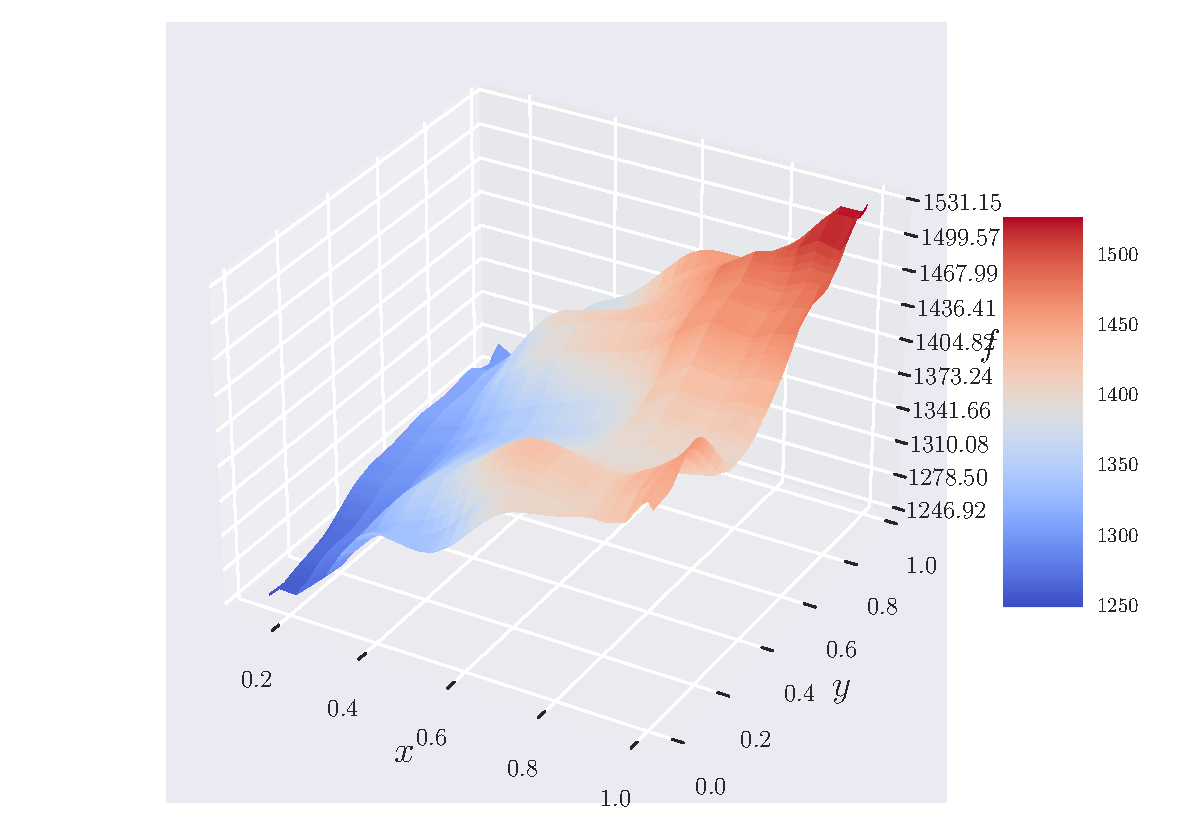
\includegraphics[width=\linewidth]{SRTM_prediction_p20.pdf}
	\endminipage\hfill
  \minipage{0.49\textwidth}
	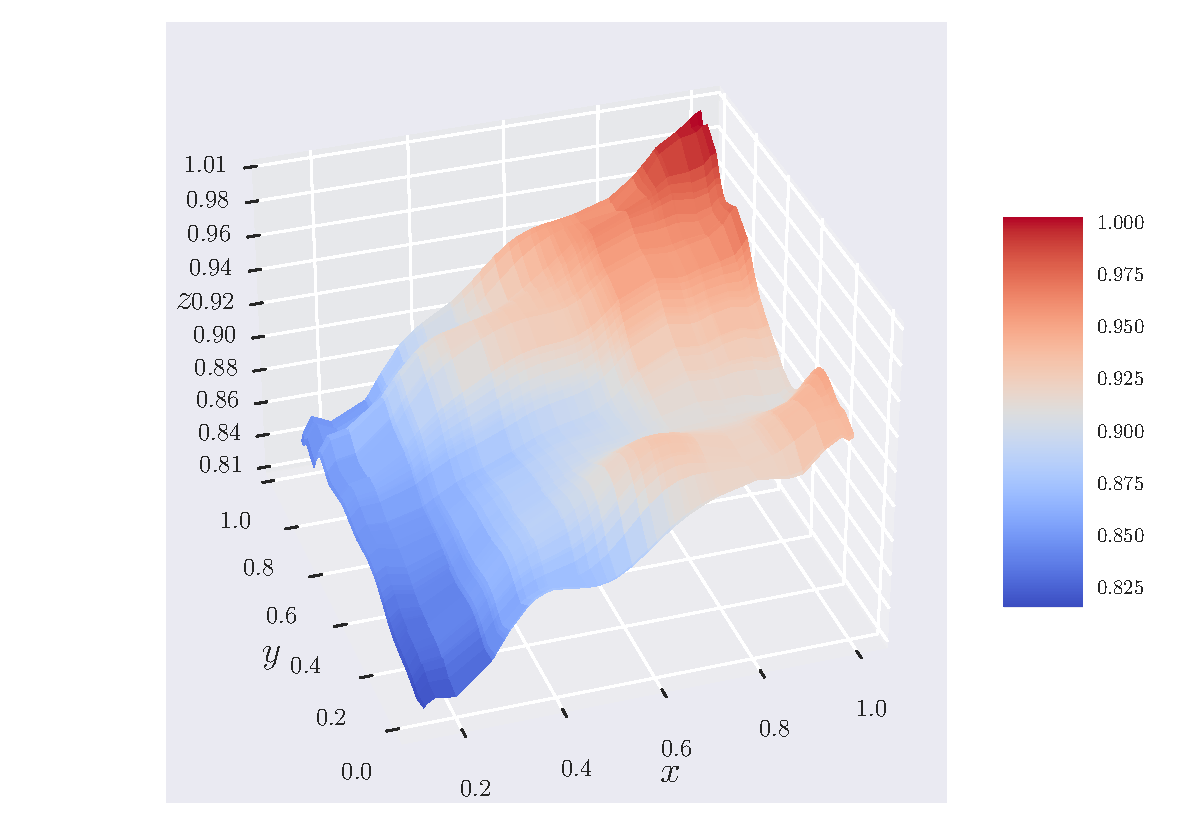
\includegraphics[width=\linewidth]{SRTM_prediction_p30.pdf}
	\endminipage\hfill
	\minipage{0.49\textwidth}
	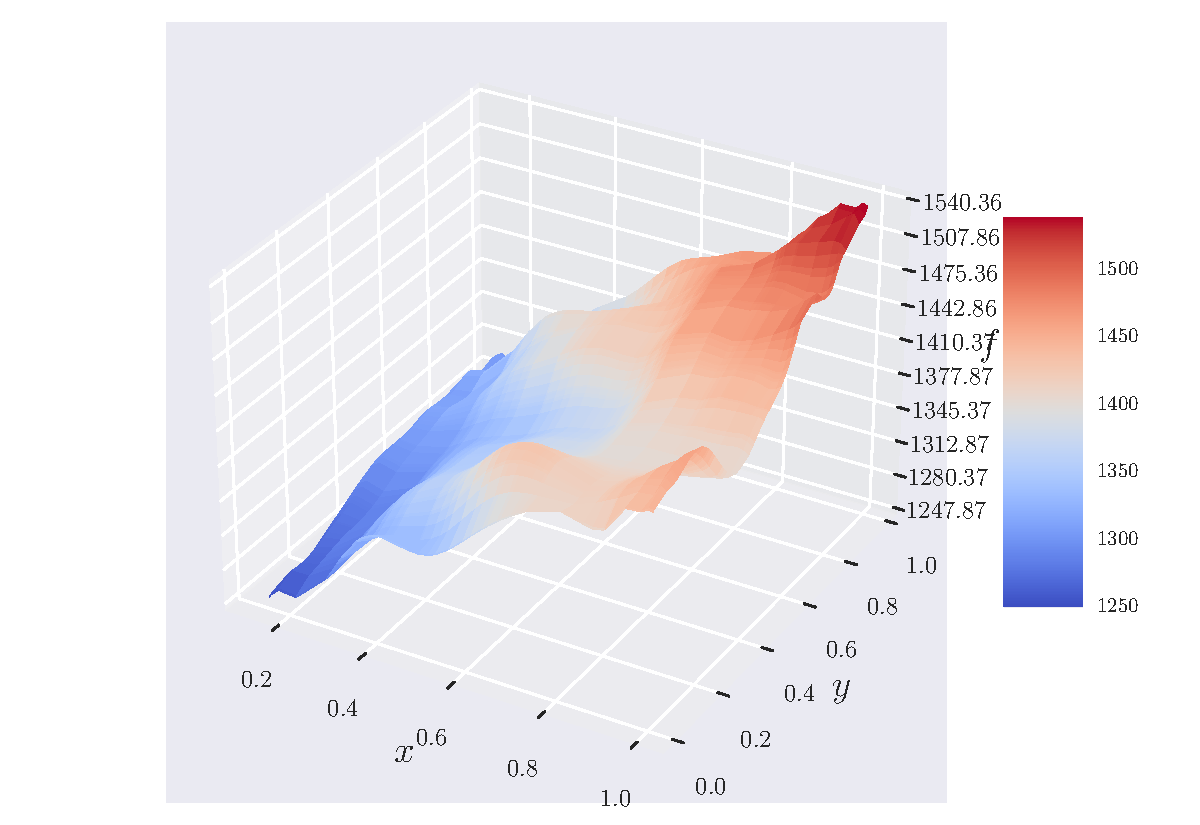
\includegraphics[width=\linewidth]{SRTM_prediction_p50.pdf}
	\endminipage
	\caption{Data til venstre. Fit til høyre}
  \label{fig:terrain_fit}
\end{figure}

In figure \ref{fig:terrain_fit} we see that $p=10$ gives a decent fit, as it captures the essential structure of the terrain. It does, however, miss out on many of the rough details in the landscape. For example the small elevation on the corner $(x,y) = (1,1)$. With $p=20$ we are able to reproduce more nuanced structures like the peak mentioned above. Increasing up to $p=30$ does not change the fit much, other than a few more details at certain points. Finally, we study the resulting fit with $p=50$. Although it provides some more rough futures of the terrain, it illustrates some difficulties of the fitting. The shape of the mountain top at $x=1$ and $y=1$ is no longer consistent with the original terrain data, and we git a tiny valley at $x=1$ and $y=0.8$, which is not an actual feature of the terrain data. Still, there are details missing along the $x$-axis at $y=1$, and the structure of the two peaks at $y=0$ is still not being represented accurately.

Next we move on to studying the MSE with cross validation. As with the bootstrap analysis, we expect the MSE to decrease in the beginning, and increase when overfitting. We use $p_\text{max} = 7$ and $k=[5,10]$ folds, and get the results shown in figure \ref{fig:terrain_OLS_MSE_CV}.

\begin{figure}[H]
	\minipage{0.49\textwidth}
	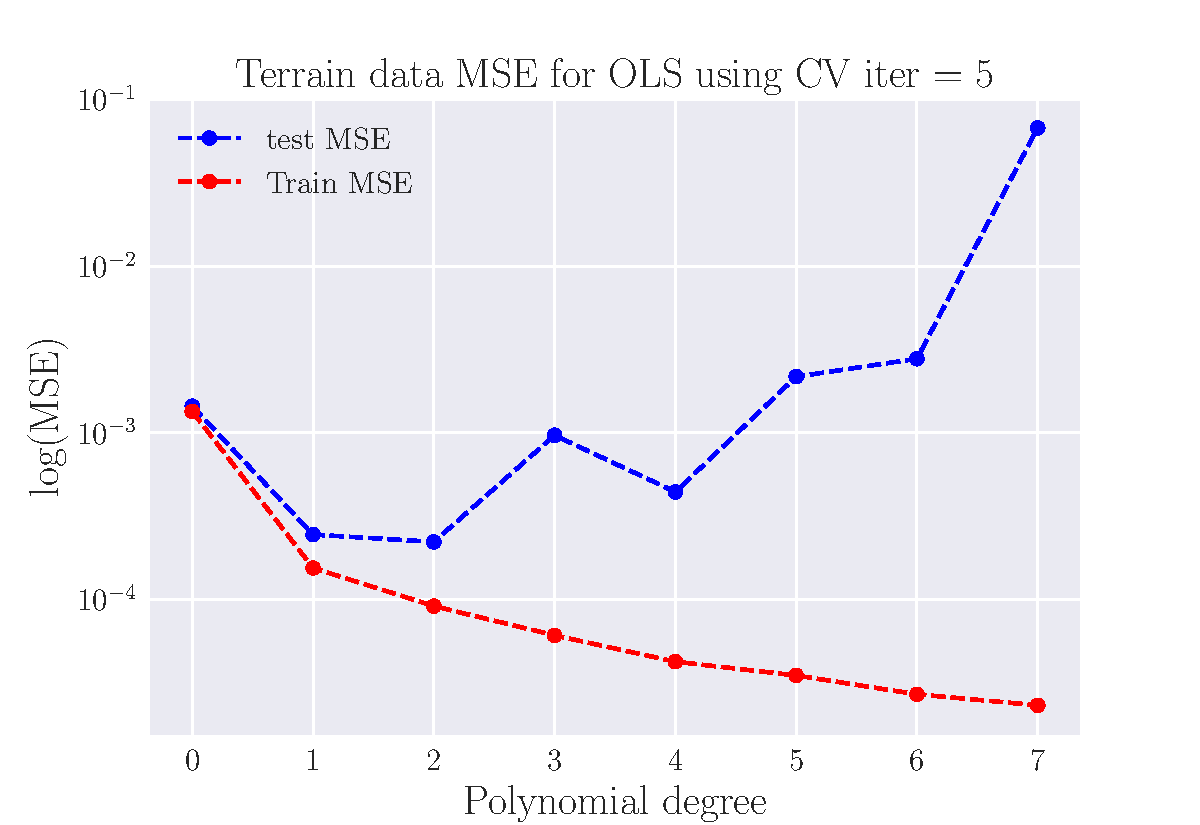
\includegraphics[width=\linewidth]{SRTM_MSE_OLS_n50_pol7_CV_re5_log.pdf}
	\endminipage\hfill
	\minipage{0.49\textwidth}
	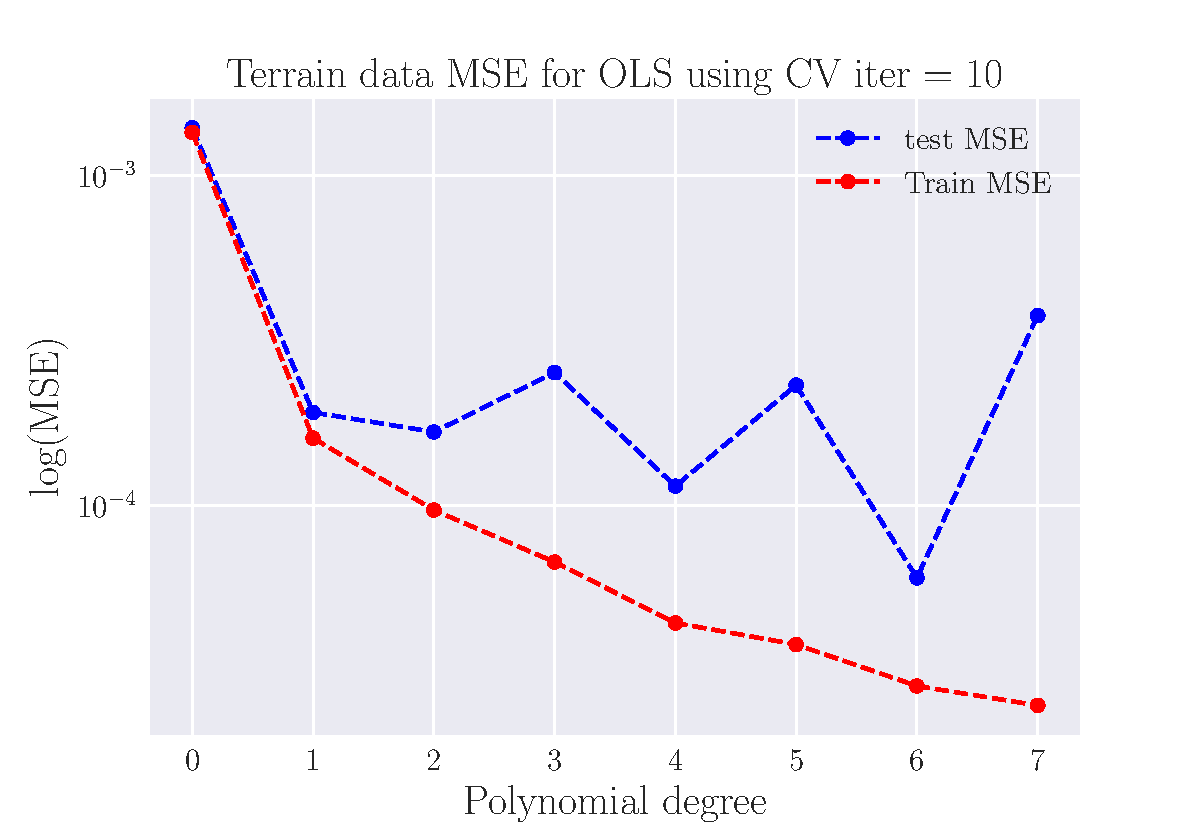
\includegraphics[width=\linewidth]{SRTM_MSE_OLS_n50_pol7_CV_re10_log.pdf}
	\endminipage
	\caption{Here we have plotted $\log(\text{MSE})$ as a function of polynomial degree, with cross-validation as the resampling technique. Left graph shows with $k=5$ iterations, and right with $k=10$.}
  \label{fig:terrain_OLS_MSE_CV}
\end{figure}
Looking at figure \ref{fig:terrain_OLS_MSE_CV} we see that the test MSE becomes large when $p>3$. Doubling the number of k-folds, the MSE drops, however the test MSE still deviates quicker, and there is a clear increase for $p>6$. Also the MSE drops much lower in figure \ref{fig:terrain_OLS_MSE_bootstrap}, almost an order of magnitude lower. There is no clear reason as to why the results are different from those obtained when bootstrapping. One reason could be that we have an "unlucky" seed, and because we have such few resampling iterations we get deviations.

Now we move on to bias-variance trade-off analysis, still expecting the same behavior as exercise 2. I.e. For both test and train, the bias and MSE should start high and variance low. The train data will get a strictly better fit for higher polynomial degree, making both the bias and MSE to decrease. For the testing data however, when we start to see overfitting (around $p=x$) variance and error should increase, while bias stays low. Using $p_\text{max}=25$,

\begin{figure}[H]
	\minipage{0.49\textwidth}
	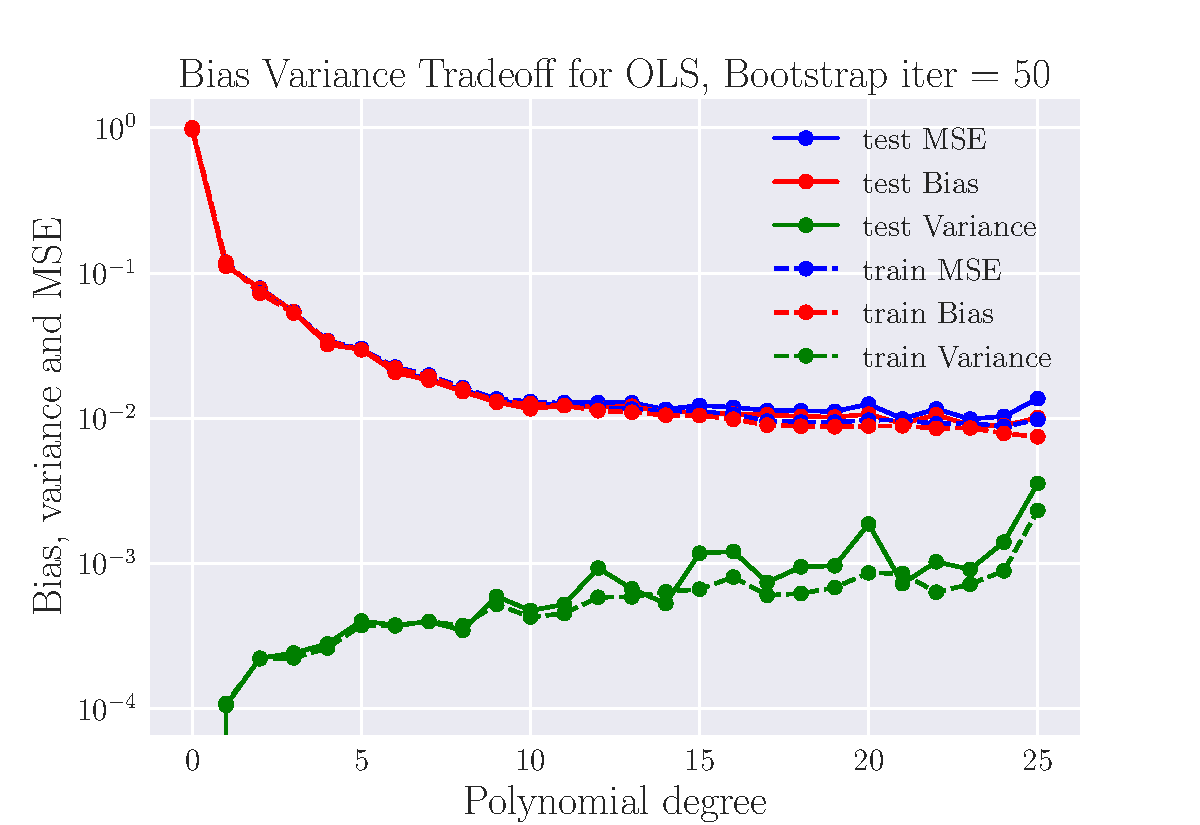
\includegraphics[width=\linewidth]{SRTM_BVT_OLS_n50_log.pdf}
	\endminipage\hfill
	\minipage{0.49\textwidth}
	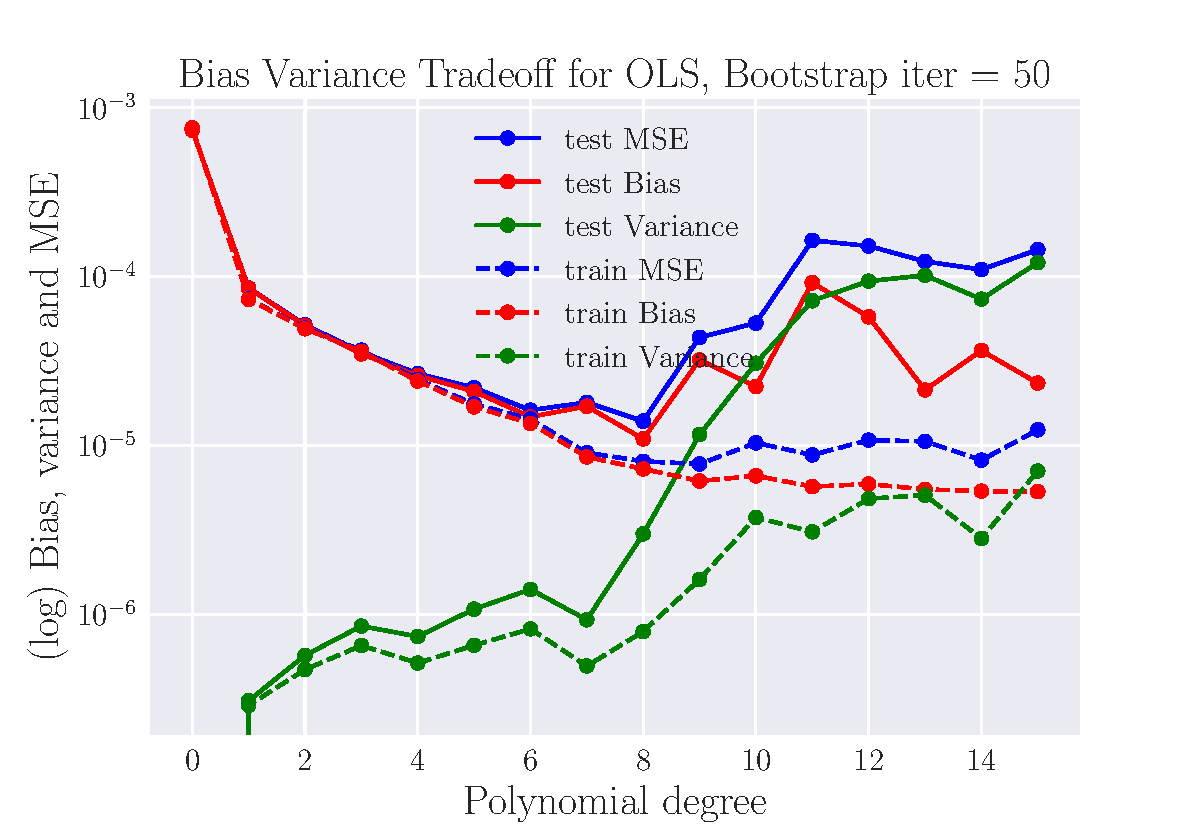
\includegraphics[width=\linewidth]{SRTM_BVT_OLS_n30_log.pdf}
	\endminipage
	\caption{Here we have plotted the logarithm of MSE, variance and bias, as a function of polynomial degree. We used $B=50$ bootstrap iterations. The left plot is with $(50\cross50)$ grid-points and right with $(30\cross30)$.}
  \label{fig:terrain_OLS_BVT}
\end{figure}

To easier see variations when we plot for $50$ data points, we use a logarithmic scale on the $y$-axis. The result is shown on the left panel in figure \ref{fig:terrain_OLS_BVT}. We see little deviations in bias and MSE, this is makes sense when considering our MSE obtained in (figure \ref{fig:terrain_OLS_MSE_bootstrap}). The test variance also deviates little from the train variance because of the same reason. Again for reference, we include the result obtained with fewer data points to see any noticeable effect. The bias-variance trade-off result for $15$ data points is shown on the right panel of figure \ref{fig:terrain_OLS_BVT}, up to $p=15$. This clearly shows the variations which we expect.

\appendix


\section{Bias-variance Decomposition}\label{Apx:BVT}

We assume that our true data is generated from a noisy model with normally distributed noise $\epsilon$ with a mean of zero and standard deviation $\sigma^2$, i.e.
\begin{align*}
  \mathbf{y} &= f(\mathbf{x}) + \bm{\epsilon}
\end{align*}

We have approximated this function with our design matrix $\mathbf{X}$ and our parameters $\bm{\beta}$ such that our model becomes $\mathbf{\tilde{y}}=\mathbf{X}\bm{\beta}$, where the values of $\bm{\beta}$ were obtained by optimizing the mean squared error via the cost function, given by

\begin{align*}
  C(\mathbf{X}, \bm{\beta}) &= \frac{1}{n} \sum_{i=0}^{n-1} (y_i - \tilde{y}_i)^2 = \mathbb{E}\left[(\mathbf{y} - \mathbf{\tilde{y}})^2\right]
\end{align*}


where $\mathbb{E}$ is the expected value. % Note sample value

We want to show that the above expression can be written as
NoteNOTE: husk å definer alt, skriv i teksten hva f, y, yhat og ytilde er!

\begin{align*}
  \mathbb{E}\left[(\mathbf{y} - \mathbf{\tilde{y}})^2\right] &= \frac{1}{n} \sum_i (f_i - \expy)^2 + \frac{1}{n}\sum_i (\tilde{y}_i - \expy )^2 + \sigma^2
\end{align*}

We begin by inserting our model expression for $\mathbf{y}$ and adding and subtracting $\expy$ inside the expected value, before we square the expression.
\begin{align*}
  \mathbb{E}\bracket{(\mathbf{y} - \mathbf{\tilde{y}})^2} &= \mathbb{E}\bracket{(f(\mathbf{x}) + \bm{\epsilon} - \mathbf{\tilde{y}} - \expy + \expy)^2} = \mathbb{E}\bracket{\closed{(f(\mathbf{x}) - \expy) + \bm{\epsilon} + (\expy - \mathbf{\tilde{y}}) }^2 } \\
  &= \mathbb{E}\bracket{(f(\mathbf{x}) - \expy)^2 + \bm{\epsilon}^2 + (\expy - \mathbf{\tilde{y}})^2} \\
  &\quad+ \mathbb{E}\bracket{2\bm{\epsilon} (f(\mathbf{x}) - \expy) + 2\bm{\epsilon}(\expy - \mathbf{\tilde{y}}) + 2 (f(\mathbf{x}) - \expy)(\expy - \mathbf{\tilde{y}})}
\end{align*}

where the cross terms have been written on a separate line since the expected value is linear. Next we will focus on the cross-terms. Since $\bm{\epsilon}$ is normally distributed, it's expected value is simply the mean, which is zero in our case. The two cross terms involving $\bm{\epsilon}$ is therefore zero, so we only need to consider
\begin{align*}
  \mathbb{E}\bracket{(f(\mathbf{x}) - \expy)(\expy - \mathbf{\tilde{y}})} &= \mathbb{E}\bracket{f(\mathbf{x})\expy} - \mathbb{E}\bracket{f(\mathbf{x})\mathbf{\tilde{y}}} - \mathbb{E}\bracket{\expy\expy} + \mathbb{E}\bracket{\mathbf{\tilde{y}}\expy}
\end{align*}
Since the expected value of an expected value is just the expected value itself the last two terms in the above equation both become $\expy^2$, canceling each other out. Using that $f(\mathbf{x})$ is a deterministic function, we have $\mathbb{E}[f(\mathbf{x})]=f(\mathbf{x})$. Expressing $f(\mathbf{x})$ in terms of its expected value, we can write the first two terms in the above equation as
\begin{align*}
  \mathbb{E}\bracket{f(\mathbf{x})\expy} - \mathbb{E}\bracket{f(\mathbf{x})\mathbf{\tilde{y}}} &= \mathbb{E}\bracket{\mathbb{E}\bracket{f(\mathbf{x})}\expy} - \mathbb{E}\bracket{\mathbb{E}\bracket{f(\mathbf{x})}\mathbf{\tilde{y}}} \\
  &= \mathbb{E}\bracket{f(\mathbf{x})}\expy - \mathbb{E}\bracket{f(\mathbf{x})}\expy = 0
\end{align*}

Hence, all the cross terms in the expected value cancel out, and we're left with
\begin{align*}
  \mathbb{E}\left[(\mathbf{y} - \mathbf{\tilde{y}})^2\right] &= \mathbb{E}\bracket{\closed{f(\mathbf{x})-\expy}^2} + \mathbb{E}\bracket{\closed{\expy - \mathbf{\tilde{y}}}^2} + \mathbb{E}\bracket{\bm{\epsilon}^2}
\end{align*}

Using that $\mathbb{E}[\epsilon^2]=\sigma^2$ and writing the expected values as sums with the notation $f(\mathbf{x}_i)=f_i$, we get the desired expression. Since we have chosen $\mathbf{z}$ as our data variable we replace all the $y$ variables with $z$, yielding
\begin{align}
  \mathbb{E}\left[(\mathbf{z} - \mathbf{\tilde{z}})^2\right] &= \frac{1}{n} \sum_i (f_i - \expz)^2 + \frac{1}{n}\sum_i (\tilde{z}_i - \expz )^2 + \sigma^2
\end{align}
which is what we wanted to show.

\end{document}
